\documentclass[12pt,letterpaper,noanswers]{exam}
\usepackage[usenames,dvipsnames,svgnames,table]{xcolor}
\usepackage[margin=0.9in]{geometry}
\renewcommand{\familydefault}{\sfdefault}
\usepackage{multicol}
\pagestyle{head}
\header{AM 108 Class 20}{}{bifurcations}
\runningheadrule
\headrule
\usepackage{graphicx} % more modern
\usepackage{amsmath} 
\usepackage{amssymb} 
\usepackage{hyperref}
\usepackage{tcolorbox}

\begin{document}
 \pdfpageheight 11in 
  \pdfpagewidth 8.5in

\noindent 




\begin{itemize}
\item There will be a pre-class assignment for Wednesday.
\item There will be a skill check in class on Wednesday.  The problem info is below.
\item Problem set 08 is due Friday October 30th.
\end{itemize}

\hrule
\vspace{0.2cm}



\noindent\textbf{Project Teams}
Team 1:


\noindent \textbf{Teams 1 and 2}: Post screenshots of your work to the course Google Drive today.  Include words, labels, and other short notes that might make those solutions useful to you or your classmates.  Find the link in Canvas (or here: \url{https://drive.google.com/drive/u/0/folders/1GcpwvKHD4tMecpFQ4lNxN_r5Ylj7YHbd})


\vspace{0.2cm}

\hrule
\vspace{0.2cm}

\noindent\textbf{Big picture}

Most of the bifurcations we have encountered involve the change in stability of a fixed point.  That means there is a straightforward way to identify the bifurcation point (by looking for the parameter value associated with a change of stability).  

There are other bifurcations, though, that are harder to detect, because they involve the birth or death of a limit cycle, which is not as easy to notice.  Those are the types of bifurcations we are learning about today.


\vspace{0.2cm}
\hrule
\vspace{0.2cm}

\noindent \textbf{Extra vocabulary / extra facts:}
\begin{tcolorbox}
A \textbf{bifurcation} is a qualitative change in dynamics that occurs with a small change in a parameter.

A bifurcation is called \textbf{local} if it can be studied via a Taylor series expansion in a small neighborhood of a location in phase space and a point in parameter space.  Examples: saddle-node bifurcation, transcritical bifurcation, pitchfork bifurcation, Hopf bifurcation

A \textbf{global bifurcation} is intrinsically nonlocal.  The \textbf{homoclinic bifurcation} is one example, as is a \textbf{saddle-node bifurcation of limit cycles}.  In this class, we are learning about a few of these global bifurcations.

\end{tcolorbox}

\vspace{0.2cm}
\hrule
\vspace{0.2cm}

\textbf{Addressing your questions}
\begin{enumerate}
    \item How does Steve determine how the amplitude and period of the bifurcations depend on $\mu$?
    
    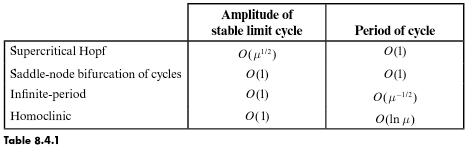
\includegraphics[width=0.8\linewidth]{img/C20limitcyclescaling.png}
    \item Saddle-node bifurcations of cycles:
    \begin{enumerate}
        \item Can the saddle-node bifurcation of cycles have the opposite stability to the one that was presented?
    \item How does $\dot r$ vs $r$ relate to the phase portraits for this?
    \item Why doesn't $\dot\theta$ also set where the bifurcation occurs?
    \end{enumerate}
    \item Would we plot bifurcation diagrams in 3d?
\end{enumerate}

\vspace{0.2cm}
\hrule
\vspace{0.2cm}


\noindent\textbf{Skill Check C21 practice}
\begin{questions}
\item Retake of skill check C18: interpreting the Poincar\'e map \emph{Note: trajectories along the line segment $\Sigma$ are not consistent with the info in the Poincar\'e map.}


\item The phase portraits below are for a system on either side of a bifurcation.
\begin{itemize}
    \item For each phase portrait, fill in the chart below.
        \item Name the bifurcation.
\end{itemize}

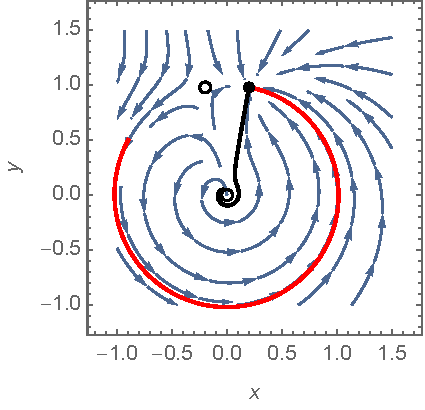
\includegraphics{img/C20-21sniperp1.pdf}
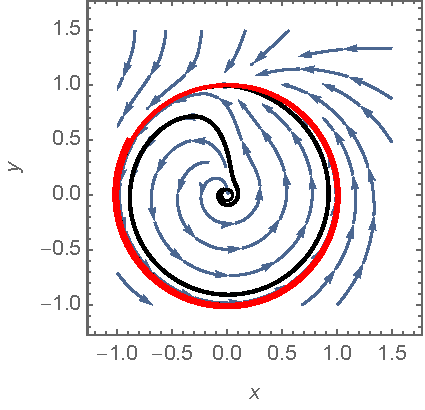
\includegraphics{img/C20-21sniperp1b.pdf}

\begin{tabular}{| c | c | c | c | c |}
\hline
plot & number of & number of  & number of  & \hspace{3in} \\
& fixed & stable & unstable &fixed point types:   \\
&  points  & limit cycles & limit cycles & attractor (a), repeller (r), or saddle (sp) \\
\hline
& & & &\\
left& & & & \\
& & & &\\
\hline
& & & &\\
right& & & & \\
& & & &\\
\hline
\end{tabular}

Name of bifurcation:

\end{questions}

\vspace{0.2cm}

\hrule
\vspace{0.2cm}

\noindent\textbf{Skill check C21 practice solution}

There is a repelling fixed point at the center in both phase portraits.  On the right, it looks like there is a stable limit cycle (and no other fixed points).  On the left, there is an attracting fixed point (and a saddle point).  It is not so visible, but it is there at about $(-0.2, 0.8)$ or so...  The pair of fixed points was born in a saddle-node bifurcation.

\begin{tabular}{| c | c | c | c | c |}
\hline
plot & number of & number of  & number of  & \hspace{3in} \\
& fixed & stable & unstable &fixed point types:   \\
&  points  & limit cycles & limit cycles & attractor (a), repeller (r), or saddle (sp) \\
\hline
& & & &\\
left & 3 & 0 & 0  & r,a,sp \\
& & & &\\
\hline
& & & &\\
right& 1 & 1 & 0 & r \\
& & & &\\
\hline
\end{tabular}

This is a SNIPer (saddle-node infinite period bifurcation).

\vspace{0.2cm}

\hrule
\vspace{0.2cm}
\noindent\textbf{Questions}

\noindent \ \ 0.  Introduce yourself to your team (and write your names on the slide).

\begin{questions}

\question (8.6.1: ``Oscillator death'' and bifurcations on a torus)  We have worked with models of a single oscillator following a reference oscillator but haven't had the chance to work with a model where each oscillator responds to the other oscillator.

This model is from Ermentrout and Kopell (1990), where the authors were considering a system of interacting neural oscillators.  They developed a simple example with two interacting oscillators that captured many of the interaction properties they wanted for their neural system.  Specifically, they wanted to capture that coupling between oscillators can actually suppress oscillation (``oscillator death'') and lead to a steady state of the coupled system.  Here is their example model:
\begin{align*}
\dot{\theta_1} = &\ \omega_1 + \sin \theta_1 \cos\theta_2 \\
\dot{\theta_2} = &\ \omega_2 + \sin \theta_2 \cos\theta_1.
\end{align*}
The oscillators have a natural frequency, but they also are responding to each other.

There are a number of different behaviors possible in this system.
We will work to figure out the possible behaviors by identifying bifurcations and  plotting a stability diagram in $\omega_1\omega_2$ space.

\begin{parts}
\item Looking for fixed points of $\phi = \theta_1-\theta_2$ allows us to identify curves where $\theta_1 = \theta_2 + c$ where $c$ is a constant. 

Here, use both $\phi = \theta_1 - \theta_2$ (``phi'') and $\psi = \theta_1 + \theta_2$ (``psi'') to aid your analysis.  

If $\dot{\phi} = 0$ and $\dot{\psi} = 0$ (and only if this is true) then the system has a fixed point.  Why is that?
\item Find $\dot{\phi}$ and $\dot{\psi}$ equations.  \emph{Look up trig identities as needed.}
\item In what region of the $\omega_1\omega_2$ plane does the system have fixed points?
\item In what regions of the $\omega_1\omega_2$ plane does this system have $\dot{\phi} = 0$ or $\dot{\psi} = 0$ but not both?  Sketch a phase portrait in the $\theta_1\theta_2$ plane in such a case.
\end{parts} 

\item (8.4.1 - SNIPer bifurcation) Consider the system given by 
\begin{align*}
\dot{r} = &\ r(1-r^2) \\
\dot{\theta} = &\ \alpha - \sin\theta
\end{align*}
with $\alpha$ slightly greater than $1$, so we are on the verge of an infinite period bifurcation.
\begin{parts}
\item Sketch the phase portrait in the $xy$-plane.
\item In lecture we saw the approximate waveform for $x(t)$.  Recall that $x = r\cos\theta$, and plot $x$ vs $t$.
\item Also sketch the waveform for $y(t)$.
\item As $\alpha$ changes so that we pass through the bifurcation, how will the amplitude of the oscillation vary with $\alpha$?
\item Let $T$ be the period of the oscillation.  If we are at a point $(x_c, y_c)$ on the limit cycle, then after time $T$, we will return to the same point.  This return takes time $T = \int_0^T dt$.  We can rewrite this in terms of our angular position on the limit cycle, so \[T = \int_0^{2\pi} \frac{dt}{d\theta}d\theta = \int_0^{2\pi} \frac{1}{\alpha-\sin\theta}d\theta.\]

We want to determine how this period, $T$, scales with $\alpha$ as we approach the bifurcation.  The bifurcation occurs when $\alpha = 1$, so we actually want to know how the period scales with $\mu = \alpha - 1$.

It is possible to use a substitution ($u = \tan \frac{\theta}{2}$) to evaluate this integral exactly.  We just want the scaling though, so we'll use an approximation.

The bifurcation occurs when $\alpha = 1$ and the system state is $r = 1, \theta = \pi/2$ at the bifurcation point.  We assume that oscillator spends most of its time close to the bifurcation.  Let $\mu = \alpha -1$ and $x = \theta - \pi/2$.  Taylor expand $\dot{\theta}$ near the bifurcation.

\emph{You should find $\dot{x} = \mu + \frac{x^2}{2}$.}

\item Assuming that most time is spent near the bifurcation, $\displaystyle T \approx \int_{-\infty}^{\infty} \frac{1}{\mu + \frac{x^2}{2}}\ dx.$  We want to rewrite this integral as $T\approx f(\mu) \int_{-\infty}^{\infty} g(x) \ dx$.  If we're able to rewrite it in that form, then $\int_{-\infty}^{\infty} g(x) \ dx$ is a constant that does not depend on $\mu$ and $f(\mu)$ tells us the scaling (how the period varies with $\mu$).

Try pulling $\frac{1}{\mu}$ out of the integral.  That doesn't quite get rid of all of the $\mu$'s.  Next try a substitution.  Let $u = x/??$ so as to eliminate the $\mu$ in the denominator.  Complete the substitution to find $f(\mu)$.  How does the period of the oscillation depend on $\mu$?

\end{parts}

\end{questions}

\eject

1: prey: $x$, predator: $y$.  fixed points: $(0,0)$, $(1,0)$, and $(a,a-a^2)$.  classification: $(0,0)$ a saddle for $a>0$, $(1,0)$ a saddle for $0<a<1$, stable for $a>1$.  $(a,a-a^2)$ unstable for $0<a<\frac{1}{2}$, stable for $\frac{1}{2}<a<1$ and a saddle for $a>1$.  Hopf at $a_c = 1/2$.   At $a_c = 1$ two fixed points exchange stability (and collide) so transcritical.  frequency of oscillation is given by the imaginary part of the eigenvalues near $a_c$ so $\omega \approx \frac{1}{2\sqrt{2}}$. Stable limit cycle at $a = 0.46, 0.48$ and stable spiral at $0.52,0.54$ so appears to be supercritical.


2a: Assume $\dot \phi = 0$ and $\dot \psi = 0$.  Then $\dot \phi + \dot \psi = 2\dot \theta_1 = 0$ so $\theta_1$ is fixed and $\dot \psi - \dot\phi = 2\theta_2 = 0$ so $\theta_2$ is fixed.  Going the other direction, if $\dot\theta_1 = 0$ and $\dot\theta_2=0$ then their sum and their difference is zero as well.

2b: $\dot\phi = \omega_1 - \omega_2 + \sin\theta_1\cos\theta_2 - \sin\theta_2\cos\theta_1 = \omega_1-\omega_2 + \sin(\theta_1 - \theta_2) = \omega_1-\omega_2 + \sin(\phi).$

$\dot\psi = \omega_1 + \omega_2 + \sin\theta_1\cos\theta_2 + \sin\theta_2\cos\theta_1 = \omega_1+\omega_2 + \sin(\theta_1 + \theta_2) = \omega_1+\omega_2 + \sin(\psi).$

2c: fixed points when $\dot \phi = 0$ and $\dot\psi = 0$ so need $\vert\omega_1 - \omega 2\vert\leq 1$ and $\vert \omega_1+\omega_2 \leq 1$.  Draw the lines $\omega_1 -\omega_2 = 1$, $\omega_1-\omega_2 = -1$, $\omega_1+\omega_2 = 1$ and $\omega_1+\omega_2 =-1$.  These lines enclose a square region (tilted 45 degrees) centered around the origin where there are fixed points.

2d: $\dot\phi = 0$ but $\dot\psi$ happens for $-1\leq \omega_1 - \omega_2 \leq 1$ and $\omega_1+\omega_2 >1$ or $\omega_1+\omega_2 < -1$.  The region between the orange and green lines below is a region where one is zero but not both.  In the $\omega_1\omega_2$ plane there are four such regions.

Assume $\dot\phi = 0$. The systems are completely decoupled, so we can just think about the $\phi$ system.  There exists a steady state $\phi$ value, $\phi_s = c$ (and usually two: one stable and one unstable).  These correspond to a steady state relationship $\theta_1 = \theta_2 + c$.  So there are two closed orbits...

\begin{verbatim}
StreamPlot[{1 + Sin[x] Cos[y], 1.5 + Sin[y] Cos[x]}, {x, -Pi, 
  Pi}, {y, -Pi, Pi}, FrameLabel -> {"\[Theta]1", "\[Theta]2"}, 
 LabelStyle -> Medium]
\end{verbatim}

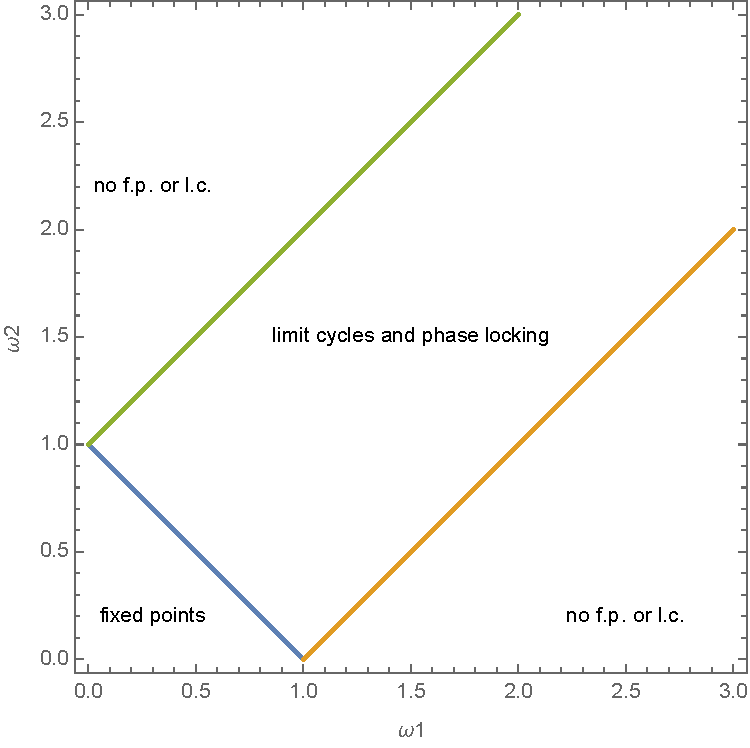
\includegraphics[scale=0.3]{img/C17plot.pdf}

2a: 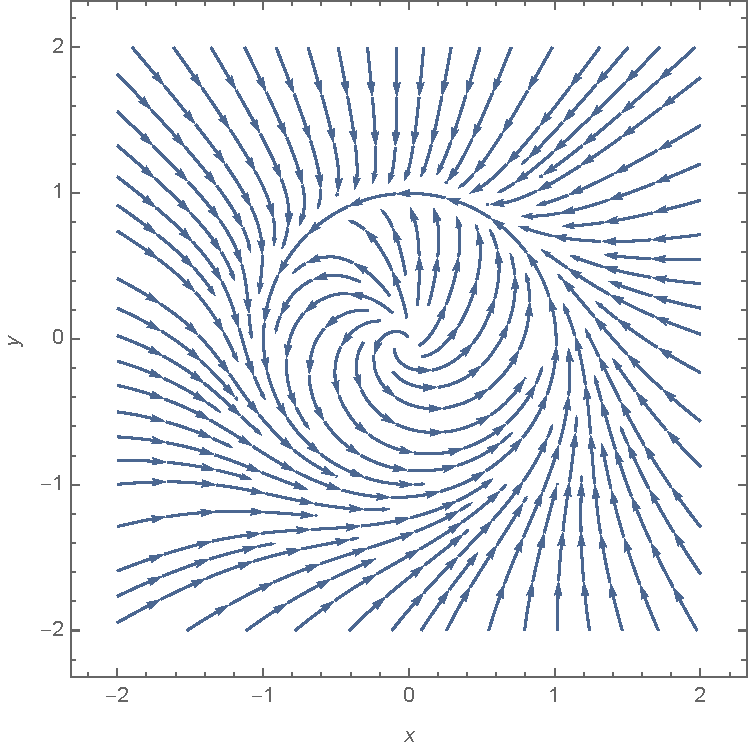
\includegraphics[width=2in]{img/C15p1.pdf}
2bc: 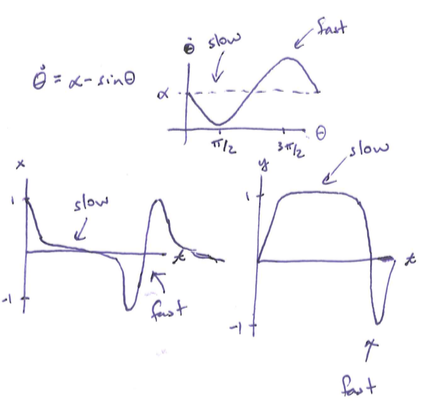
\includegraphics[width=4in]{img/S19C18p4.png}

Waveforms for $\mu = 1.1$ and $\mu = 1.01$. 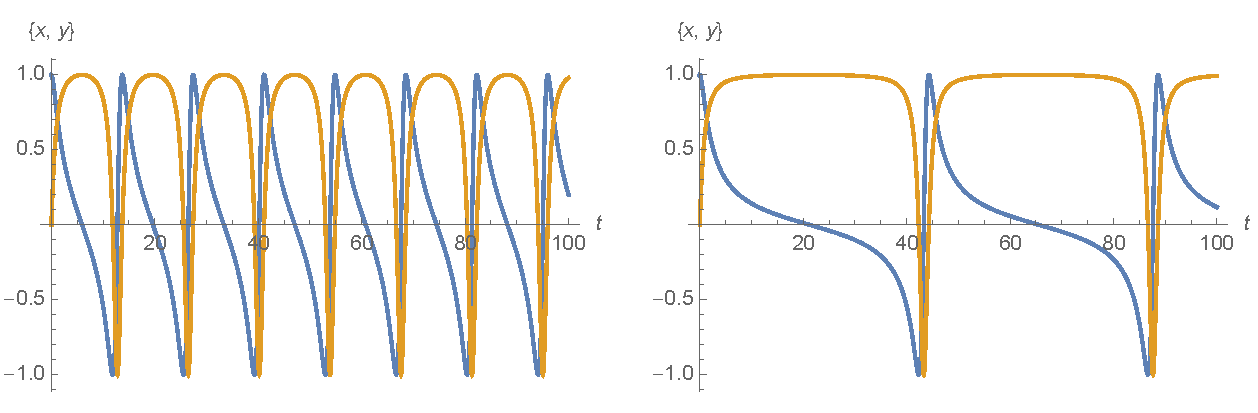
\includegraphics[width=4in]{img/InfinitePeriod.pdf}

2d: the amplitude is always about $1$, so not varying with $a$.
2e: Start with a linear approximation: $\dot \theta \approx \alpha - \sin\pi/2 + (\theta - \pi/2)f'(\pi/2) = \alpha -1 + (\theta -\pi/2)(-\cos \pi/2) = \alpha -1 = \mu$.  This isn't enough terms so go to quadratic order.  The next term is $\frac{1}{2}(\theta - \pi/2)^2f''(\pi/2) = \frac{1}{2} x^2 \sin \pi/2 = \frac{1}{2}x^2$.  $\dot \theta = \dot x \approx \mu + \frac{1}{2}x^2.$

2f: pull out $1/\mu$: $\displaystyle T \approx \frac{1}{\mu}\int_{\infty}^\infty \frac{1}{1+x^2/(2\mu)}dx$

change of variables: $u = x/\sqrt{2\mu}$ so $du = dx/\sqrt{2\mu}$.  $\displaystyle T \approx \frac{1}{\mu} \int_{\infty}^\infty \sqrt{2\mu}\frac{1}{1+u^2}du = \frac{1}{\sqrt{\mu}}\int_{\infty}^\infty \sqrt{2}\frac{1}{1+u^2}du$

\end{document}